\documentclass[a4paper,10pt]{article}

% escreve textos gerados em portugues
\usepackage[brazilian]{babel}
% aceita unicode
\usepackage[utf8]{inputenc}
% pacotes para inserção de imagens
\usepackage{graphicx}
\usepackage{epstopdf}
\DeclareGraphicsExtensions{.pdf,.png,.eps}
% pacote para fórmulas matemáticas
\usepackage{amsmath}
% pacote para row spam em tabelas
\usepackage{multirow}

\title{Comparação de algoritmos de escalonamento de workflows para redes híbridas}
\author{Aloisio Vilas-Boas\and Andre Petris Esteve\and Atilio Gomes Luiz}
\date{\today}

%% \pdfinfo{%
%%   /Title    ()
%%   /Author   ()
%%   /Creator  ()
%%   /Producer ()
%%   /Subject  ()
%%   /Keywords ()
%% }

\begin{document}

\maketitle

\begin{center}
--------------------------------------------------------------------------------------------\\
Universidade Estadual de Campinas\\
Instituto de Computação\\
MO648 - Projeto de Redes Multimídia\\
Prof. Dr. Nelson Luis Saldanha da Fonseca\\
--------------------------------------------------------------------------------------------\\
\end{center}

\section{Introdução}

Workflows científicos têm sido utilizados atualmente para representar uma grande variedade de aplicações envolvendo
alto processamento e grandes capacidades de armazenamento. Alguns domínios do conhecimento tais como a biologia estrutural,
física quântica e neurociência envolvem experimentos científicos cuja análise dos dados torna-se possível apenas por meio de sua representação
na forma de workflows científicos\cite{pso_a}.\\

Um workflow pode ser descrito como um Grafo Acíclico e Direcionado \emph{(DAG, do inglês, Directed Acyclic Graph)} no qual cada tarefa 
é representada por um nó e cada fluxo de dados entre tarefas é representado por uma aresta direcionada entre os nós correspondentes. O escalonamento 
de workflows consiste em mapear cada tarefa de um workflow para um recurso(processador) apropriado, tal que o cálculo total do mapeamento produzido 
satisfaça algum critério de performance (custo, tempo, etc). Como esse problema é bem conhecido ser um problema NP-Completo, muitas heurísticas têm 
sido propostas \cite{bit}, \cite{pso_a}, \cite{pcp}.

Dessa forma, técnicas de gerenciamento de workflows fazem-se necessárias, principalmente em ambientes distribuídos 
envolvendo serviços providos por nuvens.\\

A computação em nuvem é um novo paradigma para computação distribuída onde três tipos principais de serviços são fornecidos. São eles\footnote{http://pt.wikipedia.org/wiki/Computacao em nuvem}:

\begin{enumerate}

    \item IaaS - Infrastructure as a Service ou Infraestrutura como Serviço: quando se utiliza uma porcentagem de um servidor, geralmente com configuração que se adeque à sua necessidade.

    \item PaaS - Plataform as a Service ou Plataforma como Serviço: utilizando-se apenas uma plataforma como um banco de dados, um web-service, etc.

    \item SaaS - Software as a Service ou Software como Serviço: uso de um software em regime de utilização web.

\end{enumerate}


Em termos de disponibilidade de recursos, nós podemos classificar nuvens de Infraestrutura como Serviço(IaaS clouds) em três 
tipos diferentes \cite{hcoc}:

\begin{enumerate}

  \item Nuvens públicas: os provedores de recursos oferecem recursos de computação (processamento, armazenamento, etc) como serviços e os usuários 
  pagam por tempo de serviço utilizado. 
  
  \item Nuvens privadas: nuvens com recursos que podem ser acessados e usados por indivíduos dentro de uma organização. Nuvens privadas são 
  similares a grids privadas.

  \item Nuvens híbridas: São um misto de nuvens públicas e privadas.

\end{enumerate}

A computação por demanda oferecida pelas nuvens públicas pode ser utilizada como um recurso auxiliar para o uso de nuvens privadas (computadores, clusters e grids), 
tal que, a medida que as aplicações do cliente necessitem de recursos adicionais, esses 
recursos sejam disponibilizados pelas nuvens públicas. Contudo, a abordagem híbrida resulta em sistemas com novas demandas em gerenciamento 
de recursos. A medida que as aplicações devem lidar com nuvens públicas e privadas, um esforço adicional deve ser feito para decidir quanto 
de recurso adicional deve ser utilizado. Desta forma, todas as vezes que uma aplicação do cliente necessita de serviços adicionais 
que não podem ser fornecidos pela rede privada, a aplicação subscreve o seu pedido para para uma nuvem pública. 
Essa nuvem pública, por sua vez, fornece o serviço requerido à aplicação.\\


Um escalonador de workflows deve levar em consideração o contexto acima para tentar escalonar as tarefas do workflow de modo 
eficiente e a um custo reduzido dentro de redes híbridas. Os escalonadores de workflows podem ter diferentes políticas que 
variam de acordo com a função objetivo: minimizar o tempo de execução total, minimizar o custo total, balancear a quantidade de recursos 
usados ao mesmo tempo que alcança as restrições de deadline da aplicação, e assim por diante.

No presente trabalho, nós focamos no estudo e na implementação de quatro algoritmos para escalonamento de workflows em nuvens híbridas. 
Dois desses algoritmos (Algoritmo aleatório e Algoritmo round robin) são, de fato, bem simples e serviram para uma comparação em relação aos outros dois 
algoritmos mais sofisticados (Partial Critical Paths e Particle Swarm Optimization). Esses algoritmos foram implementados na linguagem Java utilizando como base para 
a sua implementação um simulador de nuvens chamado \emph{Cloudsim}\cite{cloudsim}.

As tarefas principais desenvolvidas neste trabalho foram:

\begin{itemize}

\item Implementação de um simulador capaz de tratar workflows em núvens hibridas, baseado no \emph{Cloudsim}.

\item Estudo e implementação de dois algoritmos de escalonamento de workflows para redes híbridas: \emph{Partial Critical Paths e
Particle Swarm Optimization}. Assim como a implementação de dois algoritmos mais simples, a saber, o algoritmo aleatório e o 
algoritmo round robin.

\item Simulação dos algoritmos e posterior comparação dos resultados. Geração de gráficos e produção de relatório.

\end{itemize}


O restante deste relatório está organizado do seguinte modo: Na seção 2 apresentamos a motivação do trabalho. Na seção 3, o contexto 
do trabalho é descrito. Na seção 4, o objetivo do trabalho é apresentado. Na seção 5, descrevemos os algoritmos que foram implementados. 
Na seção 6, descrevemos o simulador. Na seção 7, descrevemos a metodologia utilizada na realização do projeto. E na seção 8, apresentamos as conclusões.


\section{Motivação}

Podemos listar como motivações para o desenvolvimento deste trabalho:\\

\begin{itemize}

\item Rever os conhecimentos de simulação vistos na disciplina e colocá-los em prática para a resolução de um projeto real.

\item Estudar heurísticas de escalonamento de workflows e fazer sua implementação utilizando um simulador de núvens.

\item Produzir um bom trabalho visando não somente um resultado satisfatório na disciplina, mas que também possa ser útil
para responder a questão de quais são os cenários em que cada escalonador simulado aqui melhor se destaca.

\end{itemize}

\section{Descrição do contexto}

Um usuário deseja executar um workflow de tarefas representado por um \emph{grafo acíclico 
direcionado} (DAG). Cada tarefa é representada por um nó no DAG. Se uma tarefa depende de
resultados de outra tarefa, então há um arco ligando os nós das respectivas tarefas no DAG.
Um nó possui um peso relacionado ao número de intrujões necessárias para que a tarefa seja executada.
Já um arco possui um peso relacionado ao tamanho dos dados que devem ser transferidos entre tarefas
dependentes.

O usuário tem disponível uma infraestrutura de nuvem híbrida para execução do 
seu workflow. Essa infraestrutural é composta por diferentes nuvens: (a) uma nuvem 
privada, onde execuções de tarefas não acarretam custos monetários ao usuário; e (b) 
nuvens públicas nas quais o usuário paga pelo tempo de processamento utilizado.

Este usuário tem um requisito de qualidade de serviço relacionado 
ao tempo de execução do seu workflow, que chamamos de deadline. Dessa forma, o tempo 
de execução do workflow deve ser menor que o deadline.

O objetivo do usuário é realizar o escalonamento de seu DAG nos recursos da 
nuvem híbridas dentro do deadline estipulado minimizando o custo monetário.

\section{Objetivo do projeto}

Este projeto teve como objetivo comparar diferentes algoritmos de escalonamento 
para redes híbridas. Foram implementados quatro algoritmos: \emph{escalonador aleatório}, \emph{round robin},
\emph{cost-driven scheduling using partial critial paths} e \emph{algoritmo de otimização por nuvem de partículas}.
Os algoritmos são descritos na próxima seção.

\section{Descrição dos Algoritmos}
\label{algoritmos}

\subsection{Algoritmo Aleatório}

O algoritmo baseia-se na alocação aleatória de recursos para o processamento de tarefas do workflow.

Este escalonador realiza os seguintes passos:

\begin{enumerate}

    \item Realize a ordenação topológica do grafo de workflows.

    \item Enquanto o grafo for não vazio, escolha um nó sem dependentes, ou seja, uma tarefa que não possua dependências 
(ou cujas dependências já foram executadas).

    \item Aleatoriamente selecione um recurso da nuvem e atribua a execução da tarefa selecionada ao recurso.

    \item Remova o nó (tarefa) do grafo (workflow) e volte ao item 2 caso haja ainda tarefas a serem alocadas.

\end{enumerate}

O escalonador aleatório foi implementado apenas para servir como um limitante inferior para a análise.
Não esperamos que nenhum dos demais escalonadores tenha uma performance inferior ao deste algoritmo.

\subsection{Algoritmo Round Robin}

O algoritmo baseia-se na alocação sequencial de recursos para o processamento de tarefas do workflow.

Este escalonador realiza os seguintes passos:

\begin{enumerate}

    \item Realize a ordenação topológica do grafo de workflows.

    \item A cada recurso da nuvem atribua um identificador único entre 0 e N-1, onde N é o número de recursos.

    \item Defina o contador 'i' como 0.

    \item Enquanto o grafo for não vazio, escolha um nó sem dependentes, ou seja, uma tarefa que não possua dependências 
(ou cujas dependências já foram executadas).

    \item Selecione o recurso da nuvem cujo identificador é (i mod N).

    \item Atribua a execução da tarefa selecionada ao recurso obtido no item 5.

    \item Incremente o contador 'i'.

    \item Remova o nó (tarefa) do grafo (workflow) e volte ao item 4 caso haja ainda tarefas a serem alocadas.

\end{enumerate}

Este escalonador serve como base para as comparações. Espera-se que os demais algoritmos (com exceção do escalonador
aleatório) apresentem melhor performance.

\subsection{Cost-driven Scheduling Using Partial Critical Paths}

(Descrever algorítmo)

\subsection{Algorítmo de Otimização por Nuvem de Partículas}
\label{psoalgo}
A solução para o problema de escalonamento, apresentada no artigo \cite{pso_a}, é baseada numa heurística 
denominada \emph{Particle Swarm Optimization} (PSO) ou \emph{Otimização por Nuvem de Partículas}. A heurística de 
escalonamento tem como objetivo otimizar 
o custo do mapeamento tarefa-máquina baseada na solução dada pelo PSO. O processo de otimização utiliza 
dois algoritmos principais: (a) A heurística de escalonamento desenvolvida pelos autores e (b) Os passos do PSO 
para otimização do mapeamento tarefa-máquina. Antes de apresentar os algoritmos, vamos 
dar uma breve descrição do algoritmo PSO.

\subsubsection{Particle Swarm Optimization - PSO}

Particle Swarm Optimization(PSO) ou Otimização por Nuvem de Partículas é um algorítmo originalmente 
desenvolvido por Eberhart e Kennedy \cite{pso_article}. O PSO é inspirado na simulação do comportamento social de um 
bando de pássaros em revoada, com movimento localmente aleatório, mas globalmente determinado. No PSO, 
assim como em outros algoritmos, existe uma população de indivíduos, chamados de nuvem (ou enxame) de 
partículas, que em vez de utilizar operadores genéticos, evoluem através de cooperação e competição, entre si, 
por diversas gerações. As partículas se beneficiam de sua própria experiência e da experiência de outros membros 
do enxame durante a busca de um melhor fitness (alvo: comida, local para repouso, proteção de predadores, etc).

\subsubsection{Estrutura do PSO}

O PSO é muito similar a algumas técnicas da computação evolucionária, como os algoritmos genéticos, onde o 
sistema é inicializado com uma população de soluções aleatórias. Entretanto, difere dessas outras técnicas 
populacionais, pois nenhum operador inspirado pelos procedimentos de DNA, é aplicado na população, para obter 
uma nova geração de indivíduos. Em vez de mutação, são utilizadas partículas, movendo-se em um espaço de busca 
n-dimensional, sendo cada uma delas um solução potencial para o problema. Cada partícula possui também uma 
velocidade que é inicializada aleatoriamente, para que possa percorrer o espaço de soluções do problema.

A $i$-ésima partícula é representada por:
\begin{equation}
X_{i} = (X_{i1}, X_{i2},\ldots, X_{id})
\end{equation}
A melhor solução prévia, ou seja, a posição que dá o melhor valor de aptidão da $i$-ésima partícula, é registrada e representada por:
\begin{equation}
P_{i} = (P_{i1}, P_{i2},\ldots, P_{id})
\end{equation}
A taxa da mudança de posição, que é chamada de velocidade, para a partícula $i$, é representada por:
\begin{equation}
V_{i} = (V_{i1}, V_{i2},\ldots, V_{id})
\end{equation}
As partículas são manipuladas pelas seguintes equações:
\begin{equation}
v_{i}^{k+1} = w*v_{i}^k + c_{1}*rand_{1} * (pbest_{i} - x_{i}^k) + c_{2}*rand_{2} * (gbest - x_{i}^k) \label{velocidade}
\end{equation}
\begin{equation}
x_{i}^{k+1} = x_{i}^k + v_{i}^{k+1} \label{posicao}
\end{equation}

Onde:\\

\begin{description}
\item
$v_{i}^k$ - velocidade da partícula $i$ na $k$-ésima iteração\\
$v_{i}^{k+1}$ - velocidade da partícula $i$ na $(k+1)$-ésima iteração\\
$w$ – fator de inércia que determina a diversificação ou a intensificação das partículas\\
$c_{j}$ – coeficientes de aceleração; $j$ = 1,2\\
$rand_{i}$ – números randômicos entre 0 e 1; $i$ = 1,2\\
$x_{i}^k$ – posição atual da partícula $i$ na $k$-ésima iteração\\
$pbest_{i}$ – melhor posição da partícula $i$\\
$gbest$ – posição da melhor partícula da população\\
$x_{i}^{k+1}$ – posição da partícula $i$ na $(k+1)$-ésima iteração\\
\end{description}

A Equação \eqref{velocidade} é usada para calcular a nova velocidade da partícula, de acordo com sua velocidade 
anterior e as distâncias entre sua posição atual, sua melhor posição, e a melhor posição do grupo. 
A partir daí a partícula muda para uma nova posição de acordo com a Equação \eqref{posicao}. O desempenho de cada 
partícula é medido de acordo com uma função de aptidão pré-definida que é relacionada ao problema a ser 
resolvido. No nosso problema, essa função de aptidão tenta minimizar os custos das alocações dos recursos 
recursos feitas em cada partícula. No PSO, cada partícula representa uma possível solução para o problema.
Cada uma dessas soluções é refinada através de n iterações; sendo escolhida, ao final, a melhor solução de todas,
ou seja, a solução (\emph{fitness}) que possui o menor custo total.\\

Cada partícula mantém o rastro de suas coordenadas no espaço-problema, que estão associadas à 
melhor solução (\emph{fitness}) que ela tenha encontrado até então. O valor do fitness também é armazenado. 
Esse valor é chamado de \emph{pbest}. Outro valor que é rastreado é o melhor entre todos os valores, e sua posição, 
obtido por qualquer partícula na população. Esse valor é chamado de \emph{gbest}.\\

O conceito do PSO consiste a cada iteração, em mudança de velocidade, as partículas 
alcancem suas posições de \emph{pbest} e \emph{gbest}. O algoritmo PSO, tal como descrito pelos 
autores do artigo, pode ser visto nos passos abaixo:\\

\begin{description}
\item[1:] Set particle dimension as equal to the size of ready tasks.
\item[2:] Initialize particles position and velocity randomly.
\item[3:] For each particle, calculate its fitness value.
\item[4:] If the fitness value is better than the previous best \emph{pbest}, set the current fitness value as the new \emph{pbest}.
\item[5:] After Steps 3 and 4 for all particles, select the best particle as \emph{gbest}.
\item[6:] For all particles, calculate velocity using Equation \eqref{posicao} and update their positions using Equation \eqref{velocidade}.
\item[7:] If the stopping criteria or maximum iteration is not satisfied, repeat from Step 3.
\end{description}



\subsubsection{Explicação do PSO}

O algoritmo começa com a inicialização aleatória da posição e velocidade das partículas. Neste projeto, 
cada partícula representa um mapeamento tarefa-máquina, onde cada tarefa \emph{i} ($0 \leq i < \text{número de tarefas}$) representa uma dimensão da partícula
e cada dimensão recebe valores inteiros, onde cada um desses valores representa o ID da máquina para qual a tarefa $i$ deve ser atribuída.\\

Deste modo, uma partícula \emph{p} representa um mapeamento de uma tarefa para uma máquina. No nosso problema, por exemplo, se o 
algoritmo receber como entrada um workflow com 5 tarefas, cada partícula, na primeira chamada do PSO, terá 5 dimensões, que poderão variar 
a medida que o algoritmo é executado. O conteúdo de cada dimensão $i$ da partícula, ($0 \leq i < \text{número de tarefas}$), 
é o identificador(ID) da máquina para a qual a tarefa $i$ deve ser atribuída. Por exemplo, uma partícula inicial no nosso algoritmo, 
pode ser melhor ilustrada na Figura \eqref{particula}.\\

\begin{figure}[!htb]
\centering
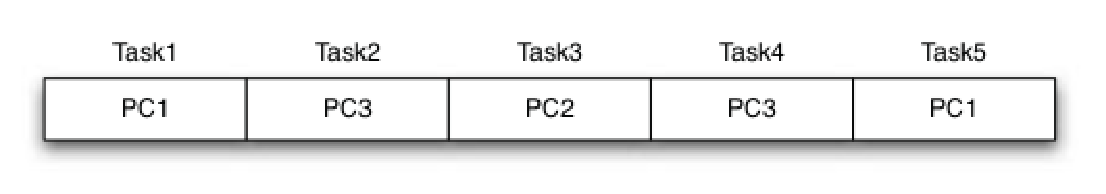
\includegraphics[scale=.5]{figures/fig1.eps}
\caption{Exemplo de partícula para um workflow com 5 tarefas}
\label{particula}
\end{figure}

\subsubsection{Explicação da heurística de escalonamento}

A heurística de escalonamento apresentada pelos autores do artigo, utiliza como recurso principal o PSO e pode ser resumida nos passos
apresentados logo abaixo:\\

\begin{description}
\item[1:] Calculate average computation cost of all tasks in all compute resources.
\item[2:] Calculate average cost of (communication/size of data) between resources.
\item[3:] Compute PSO(\emph{allTasks}) /* where \emph{allTasks} is a set of all tasks of the workflow */
\item[4:] repeat steps 5 to 10 until there are unscheduled tasks
\item[5:] for all ''ready'' tasks do: assign tasks $t_{i}$ to resources $p_{j}$ according to the solution provided by PSO
\item[6:] Dispatch all the mapped tasks
\item[7:] Wait for \emph{polling time}
\item[8:] Update the ready task list
\item[9:] Update the average cost of communication between resources according to the current network load
\item[10:] Compute PSO(remainingTasks)
\end{description}

Os valores para custo médio de computação e comunicação, assim como os valores para o tamanho 
do arquivo transmitido entre tarefas, são computados de acordo com os dados passados como entrada para o simulador.\\

O passo inicial do algorítmo é computar o mapeamento de todas as tarefas do workflow, independente das dependências
existentes entre as tarefas(passo 3: Compute PSO((allTasks)). Este mapeamento otimiza o custo total de computação do workflow. 
Para validar as dependências entre as tarefas, o algoritmo atribui as tarefas prontas para os hosts de acordo com o 
mapeamento dado pelo PSO (passo 5). Após despachar as tarefas para execução, o escalonador espera um determinado tempo, que
os autores do artigo denominaram \emph{polling time}. Esse tempo é para o simulador adquirir o status das tarefas.
Na nossa simulação, ao invés de esperar um determinado tempo, o escalonador atribui as tarefas aos hosts e continua a sua execução, sendo
avisado a qualquer momento pelo simulador(cloudsim) do término de uma tarefa. Todas as vezes que o escalonador é avisado do término de tarefas, 
o algoritmo PSO é chamado para que a geração de um novo mapeamento tarefa-máquina seja gerado (passo 7). Desta forma, o algoritmo PSO tal como
implementado pode ser denominado um algoritmo online.\\

Dependendo da quantidade de tarefas finalizadas, a lista de tarefas prontas é atualizada, essa lista conterá todas as tarefas 
cujos pais completaram sua execução e já transmitiram todos os arquivos necessários (passo 8). No passo 9, os autores 
atualizam a matriz com os valores dos custos de comunicação entre os recursos pois, segundo o modelo implementado por eles, 
esses valores podem variar. No caso da nossa implementação, esses valores são fixos, logo esse passo não precisou ser implementado 
no nosso projeto. No passo 10, o PSO é computado novamente para as tarefas que ainda não foram escalonadas. Os passos 6 a 10 
são repetidos até que todas as tarefas do worflow estejam escalonadas.\\

A Tabela abaixo mostra os valores utilizados na execução do algoritmo de escalonamento PSO. O número de execuções representa o número de 
simulações independentes realizadas para cada workflow dado com entrada para o algoritmo para se calcular o Intervalo de Confiança dos resultados.\\

\begin{figure}[!htb]
\centering
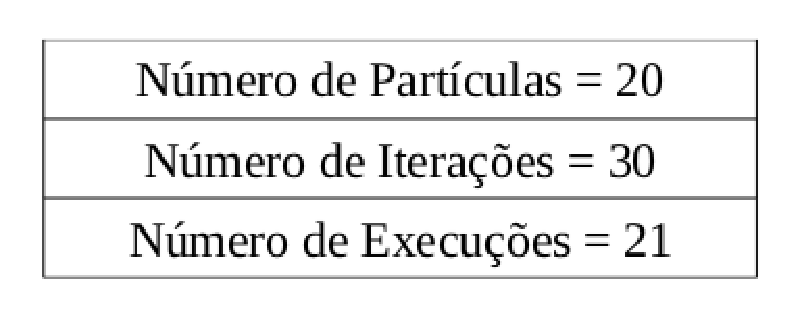
\includegraphics[scale=.4]{figures/valuesPSO.eps}
\caption{Valores utilizados no algoritmo PSO}
\label{psoValues}
\end{figure}

\section{O simulador}

Para realizar a comparação dos algoritmos, foi necessário utilizar um simulador de nuvens. O simulador é
responsável por receber e tratar os pedidos de alocação de tarefas, bem como os pedidos de transmissão dos
resultados de uma tarefa executada.

Foi implementado um simulador que atendesse aos requisitos descritos anteriormente. A implementação baseou-se
em um, já consolidado, simulador de nuvens chamado \emph{cloudsim}\cite{cloudsim}.

As alterações feitas e decisões de projeto tomadas são descritas com detalhes abaixo.

\subsection{Arquitetura}

A fim de que fosse possível testar um número variado de algoritmos e que a implementação do escalonador
não estivesse altamente acoplada ao funcionamento do simulador, decidimos adicionar uma camada de abstração
ao projeto.

Essa camada de abstração provê funcionalidades básicas ao implementador do escalonador, sem revelar como o
simulador as implementa. Desta forma, é possível alterar o simulador subjacente sem alterar o código dos escalonadores,
bem como é possível desenvolver um escalonador sem conhecer qual será o simulador utilizado.

Do ponto de vista da implementação, a camada de abstração é um conjunto de interfaces que define os contratos
entre os escalonadores e o simulador.
Ela é genérica o suficiente para permitir que diferentes escalonadores sejam suportados por diferentes simuladores.

O principal motivo dessa decisão de projeto foi permitir o desenvolvimento em paralelo da implementação dos escalonadores
e do simulador.

Portanto, a arquitetura do projeto é como vista abaixo.

\begin{center}
----------------------------------------------------------\\
                ESCALONADORES                 \\
----------------------------------------------------------\\
             CAMADA DE ABSTRAÇÃO              \\
----------------------------------------------------------\\
        SIMULADOR (CLOUDSIM MODIFICADO)        \\
----------------------------------------------------------\\
\end{center}

\subsection{Interface do escalonador}

O escalonador deve implementar uma interface que permite as seguintes
interações entre ele e o simulador:

\begin{enumerate}

  \item Inicialização
  \item Evento: fim de execução de tarefa previamente alocada
  \item Evento: fim de transmissão de dados

\end{enumerate}

Abaixo descrevemos cada possível interação entre o simulador e o escalonador.

Em (1) o escalonador deve preparar o ambiente para iniciar as alocações. Se o escalonador
não se importar com os eventos do simulador, ele pode realizar a alocação de todas as tarefas
neste momento. Nota: ao menos uma tarefa deve ser alocada nesta etapa, pois caso nenhuma tarefa
seja alocada o simulador termina, uma vez que não há o que simular.

Em (2) o simulador avisa ao escalonador que uma tarefa previamente alocada terminou sua execução.
O escalonador pode obter informações sobre o processamento, bem como alocar novas tarefas, se desejar.

Em (3) o simulador avisa ao escalonador que uma transmissão de dados terminou.
O escalonador pode obter informações sobre a transmissão, bem como alocar novas tarefas, se desejar.

\subsection{Interface do simulador}

O simulador deve, por sua vez, implementar uma interface que permite que escalonadores
realizem operações básicas durante a simulação. Essas operações são:

\begin{enumerate}

  \item Obter tarefas (DAG do workflow)
  \item Obter recursos (recursos da rede pública e privada)
  \item Alocar uma tarefa
  \item Alocar uma transmissão

\end{enumerate}

Abaixo descrevemos cada funcionalidade:

Em (1) o simulador provê o DAG que contém as tarefas, suas dependências e os pesos das tarefas (número
de instruções) e os pesos dos arcos (tamanho dos dados a serem transmitidos entre tarefas dependentes).

Em (2) o simulador provê uma lista de recursos da nuvem hibrida. Os recursos da nuvem privada diferem
dos da nuvem publica por não possuírem custo atrelado a sua utilização.

Em (3) o simulador permite que o escalonador aloque uma tarefa para execução em um recurso da nuvem.

Em (4) o simulador permite que o escalonador aloque uma transmissão de dados (resultado de uma tarefa)
entre recursos da rede. A limitação imposta aqui é que uma transmissão só é válida se ela iniciar em um
recurso que executou a tarefa cujos dados estão sendo transmitidos.

\subsection{Alterações do simulador}

Nesta seção descrevemos quais foram os requisitos que não estavam presentes no simulador original
e que foram implementados na nossa versão.

Utilizamos o \emph{cloudsim}\footnote{http://www.cloudbus.org/cloudsim/} release 2.1.1 como base para as modificações.
 
O simulador de nuvens \emph{cloudsim} não serviu imediatamente ao nosso propósito. Algumas funcionalidades
não eram implementadas ou eram parcialmente implementadas:

\begin{enumerate}

  \item Simulação da transmissão de resultados entre recursos
  \item Simular fila de transmissões
  \item Considerar dependências de tarefas antes de iniciar sua execução

\end{enumerate}

Abaixo exemplificamos cada requisito.

Considere duas tarefas A e B, sendo que B depende dos resultados de A para executar.
Considere também dois recursos $\alpha$ e $\beta$.
Se A for alocada em $\alpha$ e B em $\beta$, então antes de B iniciar em $\beta$ é necessário
que sejam transmitidos os dados gerados por A de $\alpha$ para $\beta$.

Realizar a simulação da transmissão e considerar o tempo gasto durante o processo é o
requisito descrito em (1).

Tendo em mente o exemplo anterior, suponha que foi alocada uma terceira tarefa, C, em
$\alpha$, antes que A fosse alocada. Contudo, o escalonador já previu a transmissão do
resultado de A para $\beta$. Assim é necessário manter uma fila de transmissões entre
recursos. Desta forma, é possível simular um canal entre dois recursos e garantir que
o canal realize uma transmissão por vez, bem como enfileirar transmissões requisitadas
em um canal em uso. Este é o requisito (2).

O requisito (3) é necessário uma vez que uma tarefa não pode ser executada até que todas
suas dependências tenham sido transmitidas ao recurso que realizará a execução. Desta forma,
caso uma tarefa seja alocada e suas dependências ainda não tenham terminado de ser transmitidas
a tarefa consome processamento do recurso, mas não avança sua execução.

\section{Metodologia}

\subsection{Preparação}

O experimento proposto deseja verificar a performance dos algoritmos de escalonamento
descritos na seção \ref{algoritmos}. Para isso foi estipulado um cenário padrão, que
compreende a configuração dos recursos nos quais as tarefas serão executadas.

O cenário foi definido como na tabela \ref{tab:datacenter}.

\begin{table}
\centering

  \begin{tabular}{|c|c|c|c|}  
    \hline
    Datacenter & Processadores & Processamento (kMIPS) & Custo (\$/I) \\
    \hline
    Público & 2 & 1 & 0,0000322222 \\
    \hline
    Público & 5 & 1 & 0,0000322222 \\
    \hline
    Público & 5 & 1 & 0,0000322222 \\
    \hline
    Público & 10 & 1 & 0,00007 \\
    \hline
    Privado & 10 & 1 & 0 \\
    \hline
    Privado & 15 & 1 & 0 \\
    \hline
    \hline
    Largura de banda (MB$\backslash$s)& \multicolumn{3}{|c|}{12,5} \\
    \hline

  \end{tabular}
  \caption{Configuração dos recursos no experimento}
  \label{tab:datacenter}
\end{table}

Existem dois grupos de recursos. O grupo privado é livre de custos, enquanto que o grupo público possui
um custo de utilização baseado no número de instruções executadas. 

Os custos da nuvem de recursos pública foi baseado nos custos de locação de máquinas de alto poder de
processamento providos pela Amazon EC2\footnote{http://aws.amazon.com/ec2/}.

As capacidades de processamento foram definidas com base em \cite{ips_wiki}. De acordo com \cite{ips_wiki},
um \emph{Pentium 4 Extreme Edition} é capaz de realizar aproximadamente 10 kMIPS.

Deve-se notar a diferença de capacidade de processamento entre os recursos públicos das linhas 1 e 2.
O recurso da linha 1 possui menos poder de processamento pelo menos preço do recurso da linha dois. Essa
variação foi introduzida propositalmente no experimento para acentuar a diferença entre os escalonadores.

\subsection{Experimento realizado}

Este projeto foi dividido em vários experimentos. Cada um deles consiste na execução de um conjunto (possivelmente unitário)
de DAGs. Cada conjunto é definido em (vide seção \ref{grafosusados}). Cada DAG representa um workflow.

Os grafos foram obtidos através de um gerador aleatório de DAGs. Para todos os grafos gerados,
os parâmetros abaixo foram considerados.

\begin{table}
\centering

  \begin{tabular}{|c|c|c|}  
    \hline
    \multirow{2}{*}{Número de tarefas} & Mínimo & 20\\
                                       & Máximo & 100 \\
    \hline
    \multirow{2}{*}{Custo da tarefa (kMIPS)} & Mínimo & 60 \\
                                             & Máximo & 1200 \\
    \hline
    \multirow{2}{*}{Tamanho dos resultados (kB)} & Mínimo & 10 \\
                                                 & Máximo & 10000 \\
    \hline

  \end{tabular}
  \caption{Parâmetro de aleatorização de workflows}
  \label{tab:param_workflow}
\end{table}

\subsection{Grafos usados}
\label{grafosusados}

Para o escalonador PSO (vide seção \ref{psoalgo}), que possui componentes aleatórias para o cálculo do escalonamento e
para os grafos aleatórios (vide seção \ref{grafaleatorio}), foram calculados os intervalos de confiança considerando 
95\% de nível de confiança.

Os demais escalonadores não possuem componentes aleatórias, com exceção do random. Contudo o objetivo deste último
é apenas prover um resultado de prova, a fim de ser comparado com resultados de outros escalonadores. A intenção é
verificar se nenhum escalonador comporta-se de maneira inferior ao algoritmo randômico.

Os demais grafos possuem apenas um representante no experimento, desta forma, a repetição do experimento não traria
variação nos resultados, dispensando o cálculo do intervalo de confiança.

\subsubsection{Aleatório}
\label{grafaleatorio}

Um conjunto de 21 grafos aleatórios foi gerado. Como resultado, foi considerada a média dos resultados
da simulação de cada um dos 21 grafos aleatórios.

Para todos os escalonadores, calculou-se o intervalo de confiança usando a distribuição t-Sudent com
20 graus de liberdade.

\subsubsection{AIRSN}

Vide figura \ref{airsn}.

Há apenas um grafo neste conjunto.

\subsubsection{Chimera 1}

Vide figura \ref{chimera1}.

Há apenas um grafo neste conjunto.

\subsubsection{Chimera 2}

Vide figura \ref{chimera2}.

Há apenas um grafo neste conjunto.

\subsubsection{LIGO}

Vide figura \ref{ligo}.

Há apenas um grafo neste conjunto.

\subsubsection{Montage}

Vide figura \ref{montage}.

Há apenas um grafo neste conjunto.

\begin{figure}[!htb]

\centering
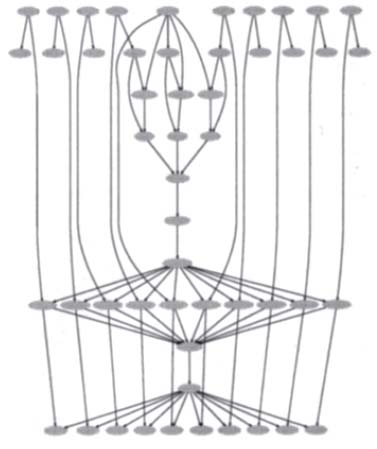
\includegraphics[scale=.25]{figures/airsn.png}
\caption{AIRSN \protect\cite{bit}}
\label{airsn}

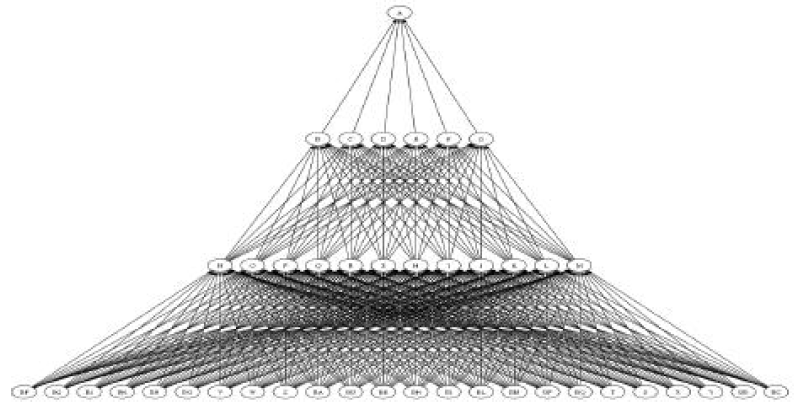
\includegraphics[scale=.25]{figures/chimera1.png}
\caption{Chimera 1 \protect\cite{bit}}
\label{chimera1}

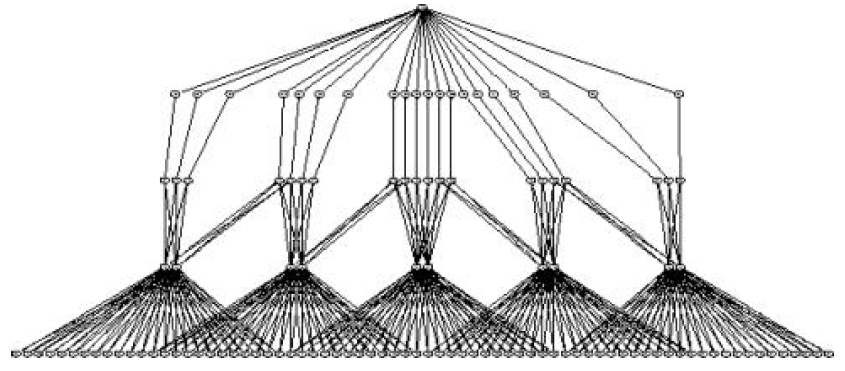
\includegraphics[scale=.25]{figures/chimera2.png}
\caption{Chimera 2 \protect\cite{bit}}
\label{chimera2}

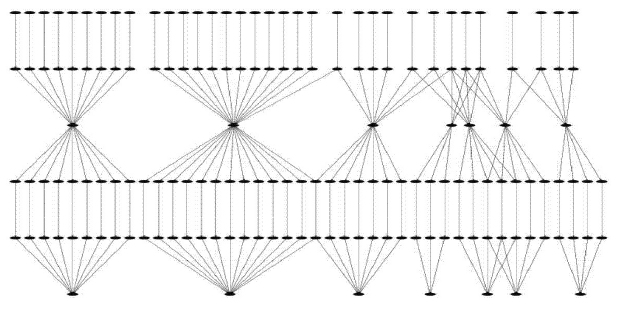
\includegraphics[scale=.25]{figures/ligo.png}
\caption{LIGO \protect\cite{bit}}
\label{ligo}

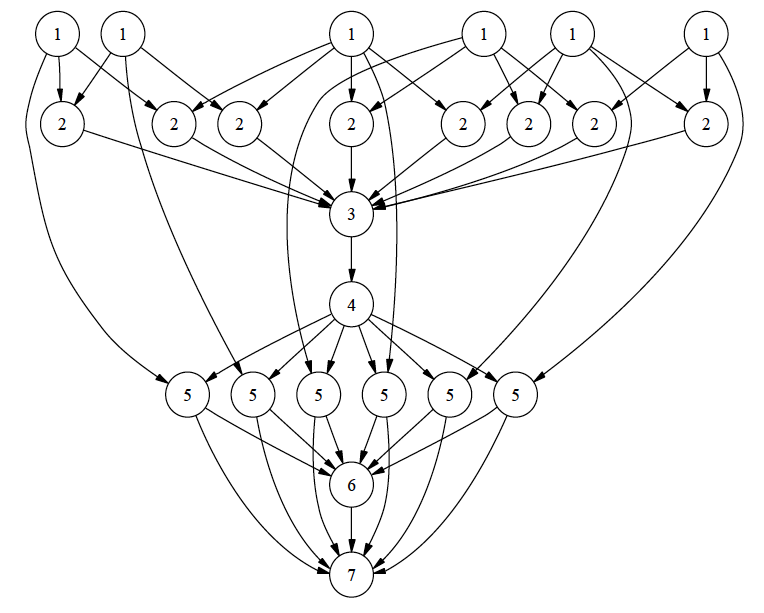
\includegraphics[scale=.25]{figures/montage.png}
\caption{Montage \protect\cite{bit}}
\label{montage}

\end{figure}

\subsection{Resultados}

De cada experimento foram obtidos dois dados. Um primeiro é o tempo, em segundos,
de execução do workflow escalonado, o outro, seu respectivo custo monetário, em 
unidades monetárias.

Assim foi possível desenhar dois gráficos de barras, para cada experimento, um
contendo o tempo de alocação do workflow, o outro seu respectivo custo. Os gráficos
foram incluídos ao final deste relatório.

Deve-se notar que há barras de erro para alguns experimentos e escalonadores,
devido aos fatores citados na seção \ref{grafosusados}. Em alguns gráficos não
é possível perceber barras de erro devido a escala utilizada. Para tais experimentos
pode-se considerar o erro associado desprezível.

Destaca-se, entre os experimentos, o relativo ao Chimera 2 (figuras \ref{chimera2_cost} e 
\ref{chimera2_time}). O tempo de execução deste workflow escalonado pelo algoritmo PSO
foi extremamente alto. Assim, devido grande diferença dos
resultados, não é possível ver no gráfico do tempo os valores obtidos pelos demais escalonadores.
Segue abaixo tais valores.

\begin{table}
\centering

  \begin{tabular}{|c|c|c|}  
    \hline
    \textbf{Escalonador} & \textbf{Custo} (\$) & \textbf{Tempo (s)} \\
    \hline
    Random & 48148.027 & 4.798 \\
    \hline
    Round-robin & 61510.473 & 6.094 \\
    \hline
    PSO & 18051.016 $\pm$ 665.137 & 91448540.479 $\pm$ 8205982.424 \\
    \hline
    PCP & 0 & 0 \\
    \hline

  \end{tabular}
  \caption{Dados da execução do Chimera 2}
  \label{tab:dados_chimera2}
\end{table}

\begin{figure}[!htb]

\centering

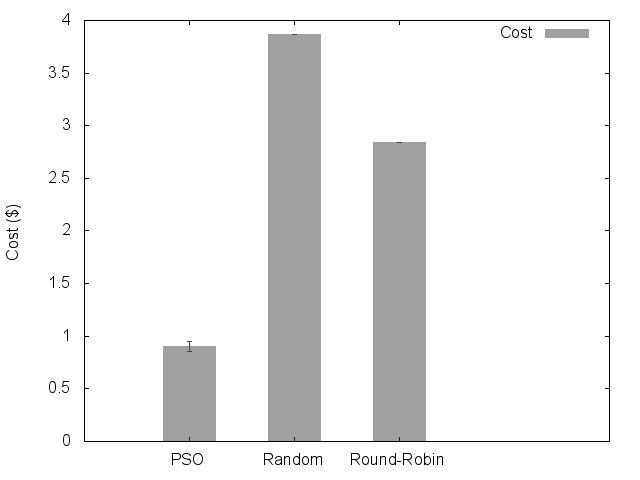
\includegraphics[scale=.55]{graphs/airns_cost.jpeg}
\label{airsn_cost}
\caption{AIRSN Cost}

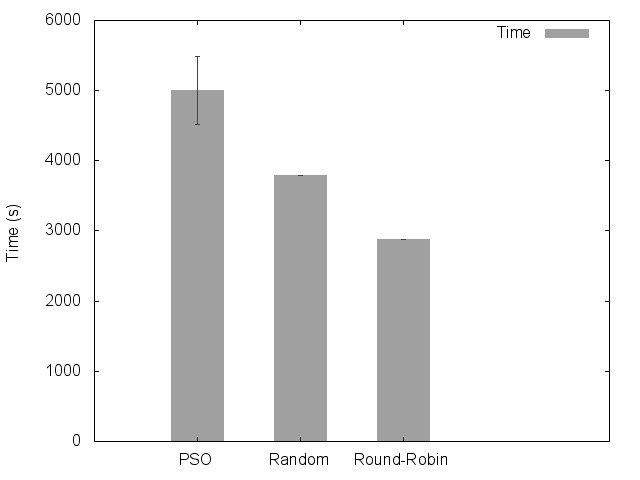
\includegraphics[scale=.55]{graphs/airns_time.jpeg}
\label{airsn_time}
\caption{AIRSN Time}

\end{figure}

\begin{figure}[!htb]

\centering

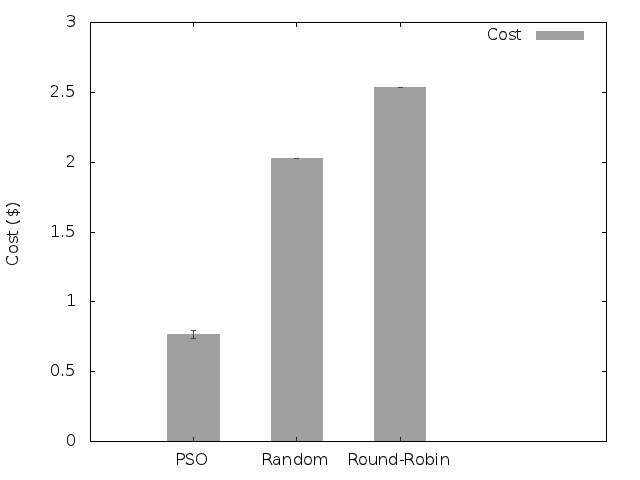
\includegraphics[scale=.55]{graphs/chimera1_cost.jpeg}
\label{chimera1_cost}
\caption{Chimera 1 Cost}

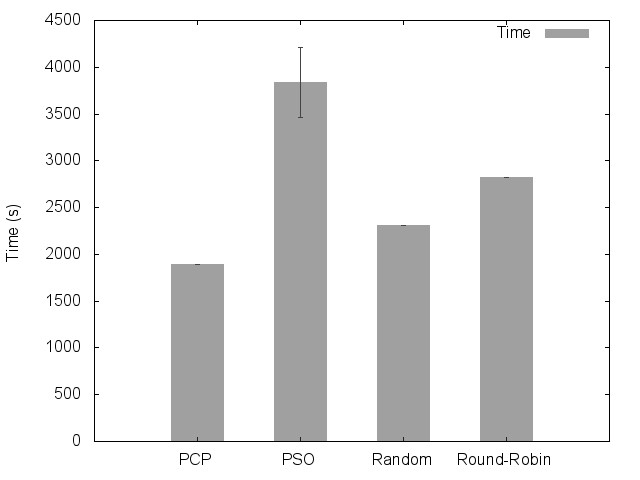
\includegraphics[scale=.55]{graphs/chimera1_time.jpeg}
\label{chimera1_time}
\caption{Chimera 1 Time}

\end{figure}

\begin{figure}[!htb]

\centering

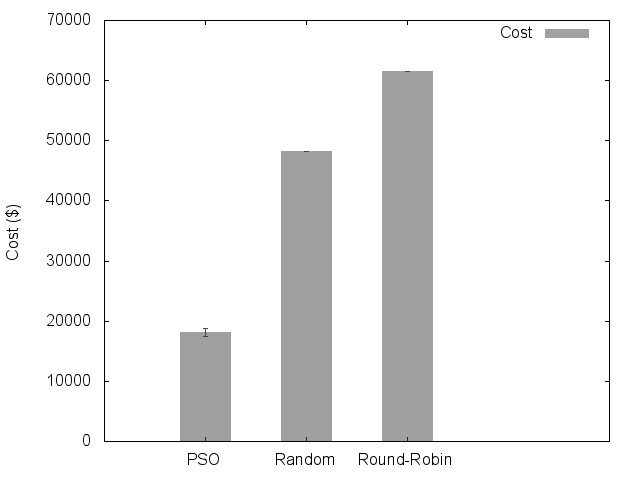
\includegraphics[scale=.55]{graphs/chimera2_cost.jpeg}
\label{chimera2_cost}
\caption{Chimera 2 Cost}

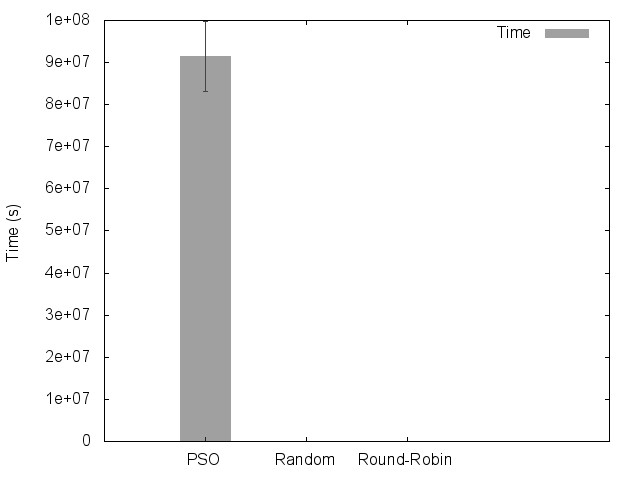
\includegraphics[scale=.55]{graphs/chimera2_time.jpeg}
\label{chimera2_time}
\caption{Chimera 2 Time}

\end{figure}

\begin{figure}[!htb]

\centering

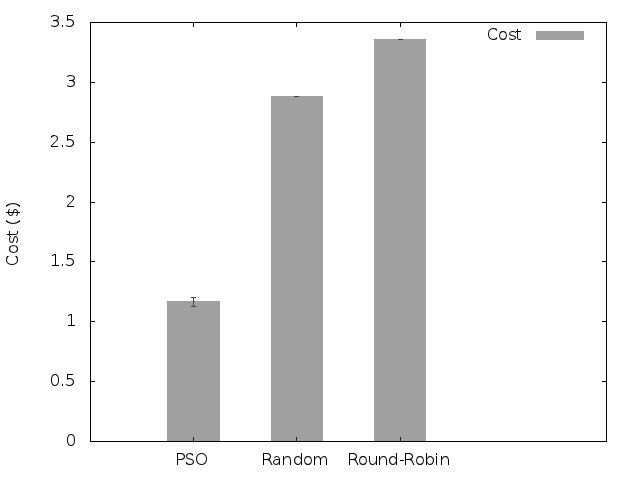
\includegraphics[scale=.55]{graphs/slideligo_cost.jpeg}
\label{ligo_cost}
\caption{LIGO Cost}

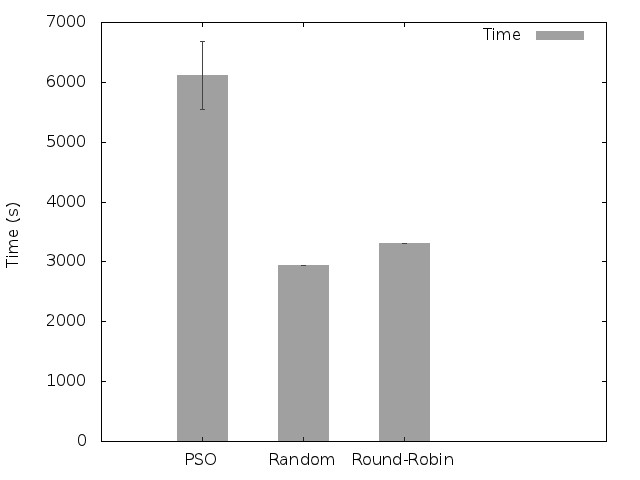
\includegraphics[scale=.55]{graphs/slideligo_time.jpeg}
\label{ligo_time}
\caption{LIGO Time}

\end{figure}

\begin{figure}[!htb]

\centering

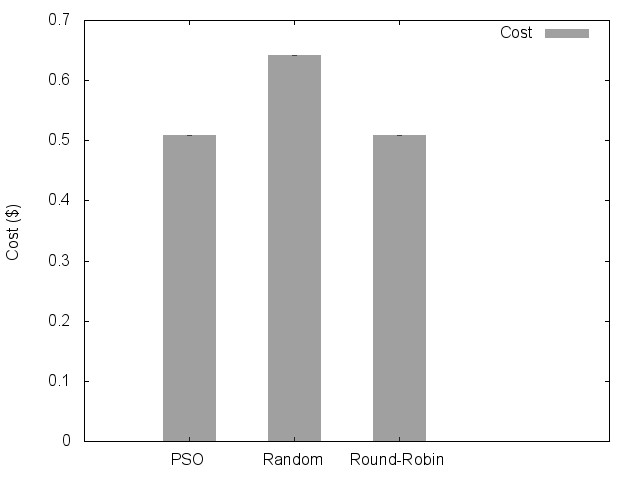
\includegraphics[scale=.55]{graphs/papermontage_cost.jpeg}
\label{montage_cost}
\caption{Montage Cost}

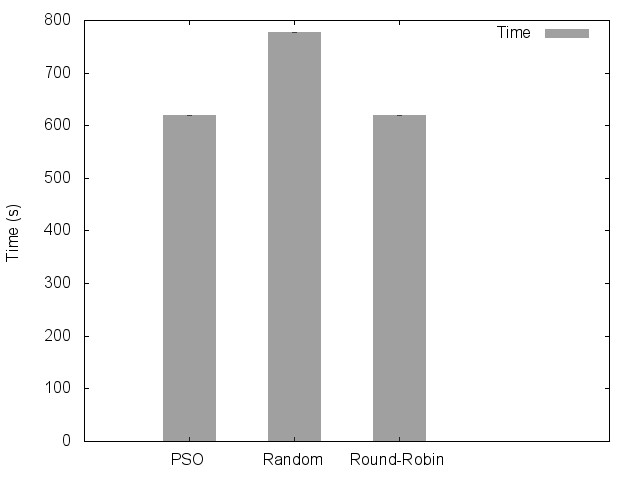
\includegraphics[scale=.55]{graphs/papermontage_time.jpeg}
\label{montage_time}
\caption{Montage Time}

\end{figure}

\section{Conclusão}

Com base nos resultados obtidos, podemos perceber que existe certa variação nos
objetivos de cada algoritmo.

Os escalonadores aleatório e round-robin serviram para o único propósito de comparar
o desempenho dos demais escalonadores, servindo como limitantes superiores para custo
e tempo.

O escalonador PSO destaca-se por obter um baixo custo de alocação, contudo por não considerar
valores de \emph{deadline} o tempo de execução das tarefas tende a ser o pior encontrado
entre os algoritmos examinados.

O escalonador PCP   8888888888complete aqui8888888888 .

Não foi explicitamente medido o tempo de execução de cada escalonador, contudo percebemos,
durante as execuções dos experimentos que, ambos PCO e PCP, demandaram algumas horas para
executar as alocações.

Dado o custo extremamente baixo exercido pela Amazon EC2, o qual foi usado como base para
o experimento, vemos que o uso de algoritmos refinados para decidir a alocação pode não ser
prático.

Desconsiderando o grafo Chimera 2, a maior diferença de custo obtida foi de aproximadamente
3 unidades monetárias (figura \ref{airsn_cost}) - o que economizou aproximadamente
25 minutos no tempo de execução do workflow (PCO x aleatório).
Dependendo do contexto, essa economia de dinheiro ou tal redução no tempo de execução pode não
ser relevante, assim deve-se examinar também em quais situações é apropriado o uso de um algoritmo
de escalonamento refinado.

Os resultados do experimento usando o grafo Chimera 2 (figuras \ref{chimera2_cost} e \ref{chimera2_time})
se mostraram os mais interessantes, uma vez que a diferença de tempo e custo obtidas entre os escalonadores
é de várias ordens de grandeza, como mostra a tabela \ref{tab:dados_chimera2}. Enquanto o escalonador PCO
conseguiu economizar aproximadamente 30 mil unidades monetárias, isso só foi possível penalizando o tempo
de execução do workflow que foi de alguns segundos para quase 4 meses.

Deve-se notar a complexidade com que as dependências ocorrem no grafo Chimera 2 (figura \ref{chimera2}).
Variações na escolha dos recursos que executarão as tarefas mais próximas à raiz pode impactar profundamente
o tempo de execução, devido a natureza das dependências do grafo. Isso explica a grande variação dos resultados
obtidos pelos escalonadores.

\section{Extensões e trabalhos futuros}

Um possível ponto de extensão a este trabalho seria examinar em quais casos torna-se relevante o uso
de algoritmos mais refinados de escalonamento. O uso do grafo Chimera 2 pode prover um bom ponto de
partida para essa análise.

\section{Agradecimentos}

Gostaríamos de agradecer a Luiz Bittencourt por nos
prover o gerador de DAGs usado nos experimentos, além de sua orientação e
conselhos, que foram fundamentais para o sucesso deste projeto.

\begin{thebibliography}{9}

\bibitem{bit}
  Luiz F. Bittencourt, Rizos Sakellariou and Edmundo R. M. Madeira,
  \emph{DAG Scheduling Using a Lookahead Variant
of the Heterogeneous Earliest Finish Time Algorithm}.
  2010 18th Euromicro Conference on Parallel Distributed and Networkbased Processing.

\bibitem{cloudsim}
  Rodrigo N. Calheiros, Rajiv Ranjan, Anton Beloglazov, Cesar A. F. De Rose, and Rajkumar Buyya
  \emph{CloudSim: A Toolkit for Modeling and Simulation of Cloud Computing Environments and Evaluation of Resource Provisioning Algorithms}.
  Software: Practice and Experience (SPE),
  Volume 41, Number 1, Pages: 23-50, ISSN: 0038-0644,
  Wiley Press, New York, USA, January, 2011.

\bibitem{pso_a}
  Suraj Pandey, Linlin Wu, Siddeswara M. Guru, Rajkumar Buyya.
  \emph{A particle swarm    optimization-based heuristic for scheduling workflow applications in cloud computing environments}. 
  In: 24th IEEE INTERNATIONAL CONFERENCE ON ADVANCED INFORMATION NETWORKING AND APPLICATIONS. Melbourn, Australia. 2010.               

\bibitem{pcp}
  Saeid Abrishami, Mahmoud Naghibzadeh, Dick Epema. 
  \emph{Cost-driven scheduling of grid workflows using partial critical paths}. 
  In: 11th IEEE/ACM INTERNATIONAL CONFERENCE ON GRID COMPUTING. October, 2010.
                                                    

\bibitem{pso_article}
   James Kennedy, Russel Eberhart. 
   \emph{Particle swarm optimization}. 
   In: IEEE International Conference on Neural Networks. 1995.

\bibitem{ips_wiki}
   Instructions per second, Wikipedia, Multiple contributors.
   \emph{http://en.wikipedia.org/wiki/Instructions\_per\_second}. 
   Último acesso em 12/12/2011.

\bibitem{hcoc}
   Luiz Fernando Bittencourt, Edmundo Roberto Mauro Madeira.
   \emph{HCOC: a cost optimization algorithm for workflow scheduling in hybrid clouds}. 2010.
 

\end{thebibliography}

\end{document}
